\section{Introduction}
\label{sec:intro}


Matrix-matrix multiplication (\textsc{GEMM}) is a key linear algebra primitive commonly used by the computational and data science communities. Examples include operations part of the setup phase of algebraic multigrid methods (AMG) \cite{Dendy82}, an example that we will use heavily in this work to demonstrate the effectiveness of our methods. It is also common for large-scale graph analytics, where a linear algebra formulation is used, such as triangle counting \cite{azad2015parallel}, graph clustering \cite{van2000graph}, breadth first search \cite{gilbert2008unified}, amongst others \cite{kepner2011graph}. 
While there are several highly-tuned distributed-memory matrix libraries available, they usually target either sparse \cite{petsc-web-page, combblas} or dense \cite{ElemNewFrame} matrices. Unfortunately, the performance and scalability of these libraries is sub-optimal for matrices that are unsupported. For the case of AMG and for graph algorithms where the linear algebra formulation necessitates a \textsc{GEMM}, the resulting matrices can lose sparsity and become potential bottleneck for performance and scalability if the underlying \textsc{GEMM} implementation is unable to handle the loss of sparsity. The main contribution of this work is the development of a scalable distributed-memory \textsc{GEMM} algorithm that is able to be performant for varying levels of sparsity.
We achieve this by developing a new divide-and-conquer \textsc{GEMM} that recursively divides the matrices vertically and horizontally. This progressively makes the matrices skinny such that the resulting product matrix block ($C = AB$) is dense. The splitting and merging of the matrices are done efficiently leveraging the sparse structure of the graphs, and aim to identify and expose dense blocks in the resulting product, for which we have implemented efficient data-structures. These product blocks are then combined in an efficient manner to produce the resulting product matrix $C$ in a sparse format. 

The divide and conquer approach improves memory access for deep-memory hierarchies, and adapts to varying levels of sparsity in a natural manner. Denser matrices will end the recursion sooner, but otherwise are identical to the behavior for sparser matrices. This enables our \textsc{GEMM} to perform in a predictable fashion independent of the density of the sparse matrix. We demonstrate the effectiveness of our algorithms and data-structures by comparing with \textsc{PETSc} \cite{petsc-web-page} and demonstrate performance comparable to \textsc{PETSc} for sparse matrices. In contrast, while the performance and scalability of \textsc{PETSc} suffers when the matrices become denser, our \textsc{GEMM} demonstrates excellent scalability even for these cases. We use the example of building an AMG grid hierarchy to evaluate our methods. Specifically, an AMG grid hierarchy is built using a Galerkin approximation by the multiplication of three sparse matrices. This leads to increasing loss of sparsity at coarser levels. Fig.~\ref{fig:sparsity} from \cite{bienz2016reducing} shows the loss of sparsity in three levels of AMG.

\begin{figure*}[hbt]
 \centering
 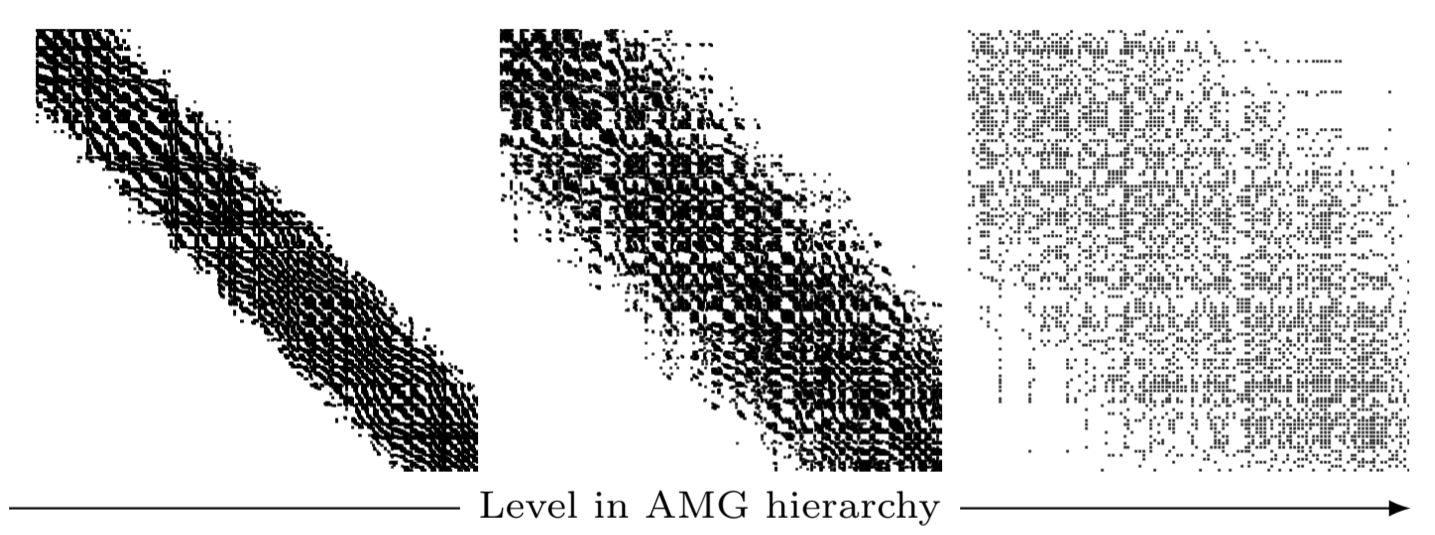
\includegraphics[width=11.8cm,height=5.4cm]{./figures/AMG_sparsity.png}
 \caption{This figure shows an example of three levels of an AMG hierarchy (levels $3$, $4$ and $5$). The loss of sparsity is noticable from this figure.}
 \label{fig:sparsity}
\end{figure*}


The main {\bf contributions} of this work are,
\begin{itemize}
  \item A new divide and conquer algorithm for \textsc{GEMM} that is able to perform efficiently for a wide range of sparsity patterns,
  \item A new communication pattern to improve the parallel scalability of \textsc{GEMM}, and
  \item A thorough evaluation and scalability study to demonstrate the effectiveness of the proposed methods.
\end{itemize}

The rest of the paper is organized as follows. In the next section, we provide background into AMG to help the readers understand the target application. We chose AMG as the application because we wanted to consider realistic scenarios where variable sparsity patterns are encountered. We provide a brief review of related work in \S\ref{sec:related}.  In \S\ref{sec:methods} we discuss the different strategies used to improve the performance and scalability of \textsc{GEMM}. In \S\ref{sec:results} we show the strong and weak scaling of our methods and compare our method with PETSc. Finally, we conclude the paper in \S\ref{sec:conc}.

\subsection{Background - AMG}
\label{sec:bg}

The solution of elliptic partial differential equation (PDE) operators forms the 
foundation of the mathematical models of several engineering applications.
In solid mechanics, the stiffness matrix derived from linear elasticity represents an elliptic
operator that, when discretized with the finite element method (FEM) yields a symmetric positive
definite system. In fluid mechanics, the viscous terms and the pressure components of
the incompressible Navier-Stokes equations, when discretized, often lead to symmetric
positive definite systems. 
For the solution of such large-scale systems that need to be solved in parallel, iterative solvers 
with $\mathcal{O}(n)$ complexity and mesh-independent convergence are preferred. 
%
The most popular methods in this regard have been the multigrid methods--both geometric and algebraic. 
The geometric multigrid (GMG) methods when applied
to matrices generated from regular (often evenly-spaced) discretizations of elliptic operators \cite{MadayMunoz88,BrambleZhang00,Brenner02,GholamiMalhotraSundar2016}.
The mathematical predictability of the benefits of the GMG approach combined with the ability to
exploit the regularity of the data structures (in terms of indexing, coarsening, etc.) has made
GMG, especially in conjunction with preconditioned conjugate gradient (PCG) \cite{Braess86,TatebeOyanagi94}, the solver of choice when solving engineering applications that require large-scale
parallel solution approaches.  The story is more mixed when one moves to unstructured discretizations
and corresponding to algebraic multigrid (AMG), the communities alternative to GMG for such problems.  

While AMG is very attractive due to its black-box nature \cite{Dendy82,Vanek:1995,VanekBrezinaMandelEtAl01}, it does not scale as well as GMG \cite{Sundar12}. This is primarily due to
the loss of sparsity at coarser levels arising from the Galerkin approximation \cite{treister2015non}, leading to poor scalability, especially at the coarser levels.
Additionally, while both geometric and algebraic variants require an initial {\bf setup} phase, the cost of the setup is significantly higher for AMG, making it less attractive unless multiple solves are performed for the same operator. This is clearly unattractive for dynamic systems where the operator is changing rapidly, such as systems with $h$ or $p$ enrichment. In such cases, while the cost of an AMG solve might be lower than say that of CG, the overall cost i.e., setup + solve might be more than using asymptotically inferior solvers. In most cases, the scalability of 
setup phase is also poor and typically worse than that of the solve phase. This has limited the attractiveness of AMG for large systems. In this work, we develop an efficient sparse matrix multiplication (\mm) algorithm to improve the performance and scalability of AMG. As will be explained in the following section, a sparse \mm\ is the dominant part of the AMG setup. While several of our optimizations apply to sparse \mm\ in general, and can be more broadly applied, our strategies for reducing inter-process communication make use of the special structure of \mm\ encountered during AMG setup.

We start with a brief description of our AMG framework. 
AMG has been a popular method for solving the large-scale and 
often sparse linear system one obtains from discretization of elliptic partial 
differential equations.  The linear system can be written as
\begin{equation}
 Ax = b
\end{equation}
\noindent in which, $A \in R^{n \times n}$, $x$ and $b \in R^{n}$.
AMG consists of a setup and a solve phase.
%Three different sets of matrices will be created during the setup phase,
%and they will be used in the solve phase to solve the linear system.
The first step of the setup phase is to aggregate the nodes of the equivalent 
graph ($G$) of the matrix $A$. Every row of the matrix $A$ is considered as a node
in the graph $G$ and there is an edge between nodes $i$ and $j$ if entry $(i,j)$ is nonzero in $A$.
%This next sentence does not make sense - "By doing the aggregation on them??".  
After aggregation, %By doing the aggregation on them, 
some nodes will be chosen as \textit{roots} and the
rest of the nodes of the graph will be assigned to them.
Multiple aggregation methods for AMG have been introduced, such as
\cite{bell2012exposing}, \cite{notay2010aggregation},
\cite{Guillard98anaggregation}, %\cite{DBLP:journals/siamsc/SalaT08}, \cite{Vanek:1995}
\cite{DBLP:journals/siammax/Notay06}. %\cite{DBLP:journals/siamsc/Notay12}, \cite{BrezinaFMMMR05}, \cite{Brezina}
For this paper, \textit{maximal independent set} from \cite{bell2012exposing}, with some modifications, is used.

Given a linear system we have $n$ 
nodes in the graph $G$ and $m$ nodes are chosen as the \textit{roots}.
We compute prolongation $P$ and Restriction $R$ operators using the \textit{roots}. 
%A matrix, called the \textit{prolongation matrix} $P$, of size $n \times m$ is defined based on these nodes. If node $i$ is assigned to root $j$, then $P(i,j) = 1$, otherwise it is $0$. The restriction matrix $R \in R^{m \times n}$ is then made by transposing $P$.
The prolongation operator has two applications. It can interpolate a vector $v \in R^m$ to $v' \in R^n$, such that $m < n$.
The other application is creating a coarse version of the operator $A$ using the Galerkin approximation:

\begin{equation}
  \label{eq:rap}
 A_c = R \times A \times P
\end{equation}

\noindent such that $A_c \in R^{m \times m}$. This operation is called \textit{coarsening}.
The restriction operator is used similarly. The triple \mm\ in (\ref{eq:rap}) is the dominant cost of the AMG setup, especially when done in parallel. Improving the efficiency and scalability of this step in the main contribution of this work. 
%; in addition to being used in the coarsening, it takes a vector $w \in R^n$ to $R^m$.

Progressively coarser versions of the matrix are created during the setup phase corresponding to
a hierarchy (i.e. multi-level or ``multigrid") of data structures.
An AMG hierarchy of $L+1$ levels consists of three categories of operators:
coarse matrices ($As$), prolongation matrices ($Ps$) and restriction matrices ($Rs$).

%\begin{enumerate}
% \item \underline{Coarse Matrices}:       $As[0]$, $As[1]$, ..., $As[L]$, where $As[0]$ represents the finest matrix $A$
% \item \underline{Prolongation Matrices}: $Ps[0]$, $Ps[1]$, ..., $Ps[L-1]$
% \item \underline{Restriction Matrices}:  $Rs[0]$, $Rs[1]$, ..., $Rs[L-1]$
%\end{enumerate}

The coarse matrices for each level are created similar to $A_c$:
\begin{equation*}
 As[l+1] = Rs[l] \times As[l] \times Ps[l],\ l = 0, 1, ..., L
\end{equation*}
such that $As[0]$ is the finest matrix $A$. Again note that this is very expensive even at the coarser levels as the matrices get denser at the coarser levels. Our \mm\ maintains good performance and scalability across all levels of the multigrid hierarchy. 

The next phase of AMG is the solve phase. To solve $Ax = b$, we start with an initial guess for $x$.
% Two methods are utilized in the solve phase to find the approximate solution:
% \begin{enumerate}
%  \item Relaxation
%  \item Coarse-Grid Correction (CGC)
% \end{enumerate}
%
% Algorithm \ref{alg:amg} shows the AMG loop, which repeats until the solution is found within the 
% desired accuracy. The grid $g$ is the AMG hierarchy, consisting the three matrix categories mentioned previously.
% %of the coarse matrices ($As$), prolongation operators ($Ps$), and restriction operators ($Rs$).
%
% \begin{algorithm}[ht] 
%   \caption{AMG} \label{alg:amg} 
%   \begin{algorithmic}[1]
%     \Require $grid\ (g)$, $b$ and $initial\ guess\ (x_0)$
%     \Ensure  $solution\ (x)$
%     \While{not converged}
%       \State $x \leftarrow\ vcycle(g,\ x_0,\ b,\ 0$)
%     \EndWhile
%   \end{algorithmic}
% \end{algorithm}
The solution is computed in a recursive function \textit{vcycle} (Algorithm \ref{alg:vcycle}).
Regular smoothers are used in the relaxation part, such as Jacobi, Chebyshev, etc.
Then, the residual $r$ is computed. Next, $r$ is taken to the coarser level by using
the restriction operator ($R$).
The function recurses until it reaches the coarsest level ($L+1$). At that level,
the system will be solved directly. The solution of that system is actually the error,
which will be interpolated by $P$.
After that, the solution will be corrected by subtracting the interpolated error from it.
Finally, the solution will be smoothed again.

\begin{algorithm}[ht] 
  \caption{vcycle($g, x,\ b,\ l$)} \label{alg:vcycle} 
  \begin{algorithmic}[1]
    \Require $grid\ g$, $b$, $x$, and $level\ (l)$
    \Ensure  $solution\ (x)$
    \If{$l = L+1$}
      \State $x \leftarrow direct\ solver(g[L+1],\ x,\ b)$
    \Else
      \State $x \leftarrow Smoother(g, x,\ b,\ l)$
      \State $r \leftarrow As[l] \times x - b$
      \State $r_c \leftarrow Rs[l] \times r$
      \State $y_c \leftarrow$ $vcycle(g, x,\ r_c,\ l+1)$
      \State $y \leftarrow Ps[l] \times y_c$
      \State $x \leftarrow x - y$
      \State $x \leftarrow Smoother(g, x,\ b,\ l)$
    \EndIf
  \end{algorithmic}
\end{algorithm}

\textit{Smoothed Aggregation AMG (SA-AMG)}\cite{Vanek:1995} is a modified version of AMG,
in which the prolongation and restriction operators are smoothed %, for instance by the Jacobi method,
to improve the convergence of AMG.
For this paper, the improved version of SA-AMG in \cite{treister2015non} is used.


\subsection{Related Work}
\label{sec:related}

While significant research has been done on improving the efficiency and scalability of sparse matrix-vector products, sparse \mm\ in comparison has received far less attention. Yuster and Zwick \cite{Yuster2005} provide a theoretically nearly optimal algorithm for multiplying sparse matrices, but rely on fast rectangular matrix multiplication. Consequently the approach is currently of only theoretical value. In \cite{Buluc12}, Buluc and Gilbert present algorithms for parallel sparse \mm\ using a two-dimensional block data distributions with serial hypersparse kernels. 
Gremse {\em et al.} \cite{Gremse15} present a promising algorithm using iterative row merging to improve the performance on GPUs. Similarly, Saule {\em et al.} \cite{Saule14} evaluate the performance of sparse matrix multiplication kernels on the Intel Xeon Phi. Most AMG implementations have relied on standard sparse \mm\ implementations without any special considerations for the structure of the matrices generated within AMG. This work attempts to fill this gap. 


%\mr{expand this section if possible.}




% \begin{itemize}
%   \item \st{General intro to AMG and elliptic operators, black box nature.}
%   \item \st{General outline of AMG method, setup and solve.}
%   \item \st{Why setup costs are important, what dominates}
%   \item what others have done.
%   \item This work and contributions.
%   \item rest of the paper.
% \end{itemize}
